Data today is growing in both size and variety. By modeling the data within a data cube based framework, it is possible to tame the vast collection of various representations of complex data into a predictable structure. This simplified data model imposes structural restrictions on the data, and in doing so makes the data more amenable to interactive visual analysis.

\section{Contributions}

The contributions of this dissertation are novel data structures and algorithms covering a broad range of the data visualization pipeline. The Universal Data Cube data model is an attempt at providing a data model that both captures the essence of many data sets and exposes a simple and predictable data structure upon which interactive visualization systems can be built. The Reactive Visualization approach is the first to synthesize the Model View Controller paradigm with functional reactive programming to construct reusable interactive visualization components. Dynamic visualization configuration allows reusable visualizations to be instantiated within the context of many data sets and allows users to collaborate in real time over interactive visualizations. Taken together, these contributions represent a new approach to the process of integrating and visualizing data.

Reactive models provide the foundation for reactive visualizations. This approach allows the construction of reusable reactive flows that encapsulate elements of interactive visualizations. Using reactive flows, much of the data visualization pipeline can be implemented. Reactive flows enable representation of update flows from data and configuration through to visualization scales, axes and visual marks. In theory, any imaginable visualization technique can be implemented as a reactive visualization component. The prototypes presented in this dissertation serve as a starting point for a growing catalog of Open Source visualization modules.

Interactions such as brushing, picking and zooming can also be encapsulated using reactive models. The interactions in one visualization can be used to drive interactive changes in other visualizations. In this way visualizations with multiple linked views can be constructed. Interaction schemes for linked views include dynamic filtering, slicing, linked selection and linked probing. For example, zooming in a map can filter the regions used to filter the input to a line chart of population. This technique of using interaction for dynamic slicing can be used to build data cube exploration tools that replace small multiples with interactive linked views.

An application state model based on reactive models provides the foundation for a collaborative visual data exploration platform. Application state configuration based on JSON enables configuration of visualizations with multiple linked views. A unique runtime engine is introduced for configurable applications that dynamically loads required modules. Using this framework it is possible to author and evolve instantiations of reusable visualization components with linked views. The application state model also affords construction and navigation of history graphs supporting undo, redo, and view sharing.

The Universal Data Cube framework proposes a framework for representing data based on the data cube model. This framework is ``universal'' in that it is capable of representing aggregated summaries of any measurable quantity over limitless time and space. The Time and Space dimensions provide conceptual delineations between regions of hierarchical time and space. Measures provides windows into phenomena occurring within certain regions of time and space. In theory, all measurable quantities that summarize events and phenomena can be represented using this framework. The limited Open Source proof of concept implementation of the UDC framework is proposed as the seed for a large ongoing project aimed at curating and exposing public data.

By combining the data curated within the UDC and the proposed visualization and collaboration frameworks, the aim is to provide a complete platform for data visualization. The hope is that this platform will enable Web users and content creators to easily investigate any data of interest using interactive data visualization. Application areas for this technology include commercial data analysis, business intelligence, education, journalism and public policy.
% Notes from 10/9 Haim MTG
% Collaboration real contributions? Talk more about collaboration.
% This is marketing "I've done something that is new"
% Brag about it.

% What one could have done but I didn't do.

\section{Future Work}
The realization of this work so far is far from the complete vision. The vision is to establish a Wikipedia-like platform for collaborative data visualization. The technologies presented in this dissertation provide the foundation for such a system, but more work needs to be done to glue the pieces together into a complete and coherent suite of tools.

The reactive model solution introduced has the potential to be formalized as a time tick based execution system. This kind of formalization would allow a rigorous asymptotic analysis of reactive models based on their data flow graph structure. For example, one could quantify the influence of various graph characteristics such as total number of nodes and breadth first search tree distance from a node that is the source of a change. 

The Universal Data Cube data model has the potential to be implemented within a database. This would involve the construction of a database schema that persists the UDC model and allows users to query the data present. The overall effect of maintaining a UDC database is that common dimensions and measures will become clear. Given a collection of 100 data sets, a UDC database could keep track of the total list of all dimensions and all measures. For each dimension, the database could tell you how many data sets use it, and what the most common key codes are. The database could also provide information about measures such as how many measures there are, how many data sets cover each measure, and what dimensions and members are covered by each measure. These kinds of queries could be coupled with visualization interfaces to present a rich overview of a large collection of data and support unprecedented visual data exploration capabilities.

The envisioned collaboration framework would be a database driven Web application enabling users to import their own data, add their own reusable visualization components, and collaboratively author interactive visualizations. User interfaces supporting these operations must also be developed. For importing data sets, a simple solution similar to the ManyEyes data import user interface would suffice \cite{viegas2007manyeyes}. For adding reusable visualization components, an in-browser code editing tool with versioning would be required (similar to JSBin). For collaboratively authoring interactive visualizations, the dynamic configuration structure can be linked with an operational transformation system such as ShareJS or Firebase. States of interest must be persisted to a database for later viewing or further editing. Existing collaboration platforms that already track data sets such as OpenChorus \cite{openChorus} could be extended to include interactive visualizations. The visualization state created by users can be simply persisted as a string in the application database.

The UDC visualization technology can be extended to accommodate real time updating data. This could be accomplished by polling for data updates or using a server push technology such as WebSockets. For updating data, the data values of the most recent time slice of the data cube may change. For granular time slices such as hours or days, new Time dimension members are created as time passes, so new slices of the data cube could be sent from the server to clients as they become available.

Mobile technology could be one of the largest targets for interactive visualization technology. For example, many readers of popular news feeds such as the New York Times consume their content using mobile devices such as smart phones, phablets and tablets. The same is true for E-Books and blogs. With this in mind, considerations must be made regarding how to tailor the proposed interactive visualizations to mobile devices with touch screen interfaces and variable resolution.

Only a few reusable visualization components have been implemented and a few data sets imported into the framework so far. The following sections discuss development of more reusable visualization components, more interaction techniques, and importing of more data sets into the UDC framework.

\section{Visualizations and Interactions}
The complete set of visualization techniques suitable for adaptation as reusable components is vast. Bertin enumerates the numerous possibilities for visually encoding data \cite{bertin1983semiology}. This is why an expandable user-driven platform is more suitable than a fixed set of visualizations. As a first step toward the goal of an open platform with the potential to accommodate any imaginable visualization technique, an initial set of visualization techniques are presented here in table \ref{table_data_cube_visualizations}.

These visualizations can be augmented by interaction techniques such as brushing, picking, hovering, pan and zoom. Each of these interactions results in a user defined subset of the data visualized. The output from the interaction in any visualization can be used to slice or filter the input of another. Brushing involves the interactive visual definition of a rectangular region that defines intervals in data space. The intervals defined by a brush region can be used to filter the original data, allowing users to interactively define subsets of the data. Picking involves tapping or clicking on a single visual mark. Hovering (also called probing) selects the single visual mark closest to the mouse. Hovering can use a Voronoi overlay to improve performance. Panning and zooming can be used on a geographic map to define a subset of regions. Conceivably, pan and zoom could also be implemented in other visualizations such as scatter plot.
\newcommand{\thumbnailWidth}{1.2in}
\newcommand{\descWidth}{2.9in}
\newcommand{\descPadding}{\vspace{.3\baselineskip}}

\begin{table*}
  \caption{Reusable Data Cube Visualizations.}
  \centering
  \label{table_data_cube_visualizations}
  \begin{tabular}{ | c | c | c |}
    \hline
    \textbf{Name}
      & \textbf{Thumbnail}
      & \textbf{Description} \\ \hline

    Bar Chart

      & \parbox[c]{\thumbnailWidth}{\centering 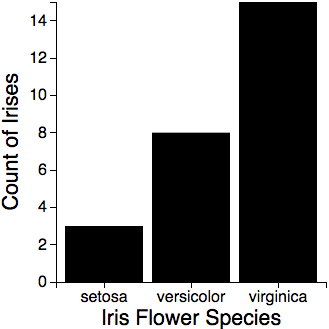
\includegraphics[width=\thumbnailWidth]{figs/visThumbnails/barchart.png}}
      & \parbox[c]{\descWidth}{\descPadding
        1 Dimension (bar) \\
        1 Measure (bar height) \\
        Optionally: \\
        Picking interaction (click on bar)
      \descPadding} \\ \hline

    Pie Chart

      & \parbox[c]{\thumbnailWidth}{\centering 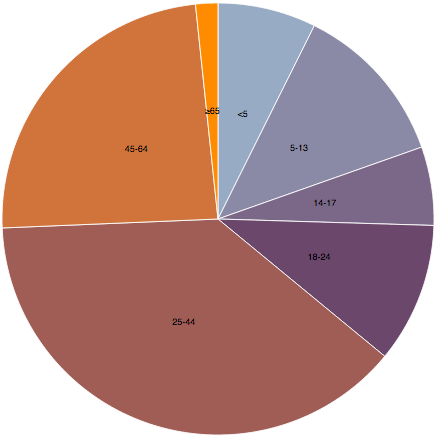
\includegraphics[width=\thumbnailWidth]{figs/visThumbnails/pie.png}}
      & \parbox[c]{\descWidth}{\descPadding
        1 Dimension (slice) \\
        1 Measure (slice size) \\
        Optionally: \\
        Picking interaction (click on slice)
      \descPadding} \\ \hline


    Scatter Plot

      & \parbox[c]{\thumbnailWidth}{\centering 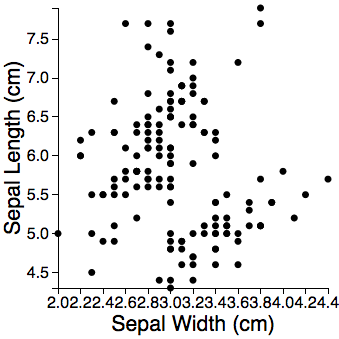
\includegraphics[width=\thumbnailWidth]{figs/visThumbnails/scatterplot.png}}
      & \parbox[c]{\descWidth}{\descPadding
        1 Dimension (mark) \\
        2 Measures (X, Y position) \\
        Optionally: \\
        +1 Dimension (symbol) \\
        +1 Measure (size) \\
        +1 Measure (color) \\
        Brushing interaction (2D)
      \descPadding} \\ \hline

    Parallel Coordinates

      & \parbox[c]{\thumbnailWidth}{\centering 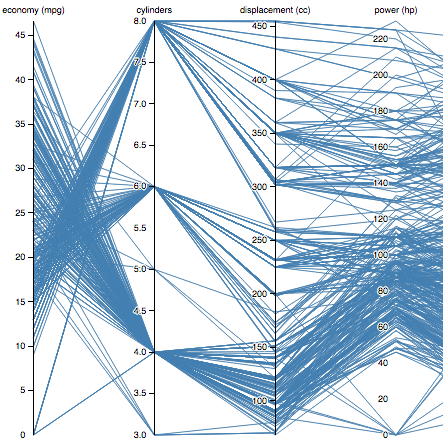
\includegraphics[width=\thumbnailWidth]{figs/visThumbnails/parallelCoords.png}}
      & \parbox[c]{\descWidth}{\descPadding
        1 Dimension (polyline) \\
        N Measures (one for each parallel axis) \\
        Optionally: \\
        Brushing interaction for each axis
      \descPadding} \\ \hline

    Choropleth Map

      & \parbox[c]{\thumbnailWidth}{\centering 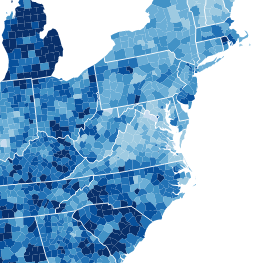
\includegraphics[width=\thumbnailWidth]{figs/visThumbnails/choropleth.png}}
      & \parbox[c]{\descWidth}{\descPadding
        1 Dimension, Space (geographic region) \\
        1 Measure (color) \\
        Optionally: \\
        Small multiples visualization overlay \\
        Picking interaction (click on region) \\
        Pan \& Zoom interaction
      \descPadding} \\ \hline
  \end{tabular}
\end{table*}

\begin{table*}
  \caption{Reusable Data Cube Visualizations (continued).}
  \centering
  \begin{tabular}{ | c | c | c |}
    \hline
    \textbf{Name}
      & \textbf{Thumbnail}
      & \textbf{Description} \\ \hline

    Sunburst

      & \parbox[c]{\thumbnailWidth}{\centering 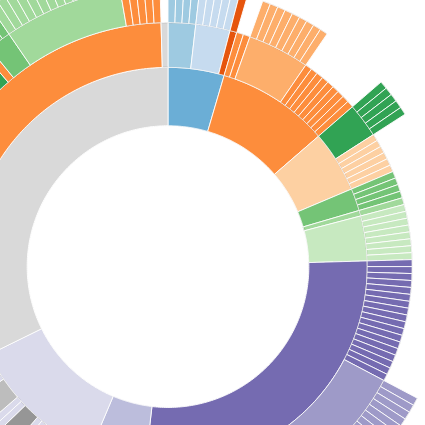
\includegraphics[width=\thumbnailWidth]{figs/visThumbnails/sunburst.png}}
      & \parbox[c]{\descWidth}{\descPadding
        1 Dimension, Hierarchical (slice) \\
        1 Measure (slice size) \\
        Optionally: \\
        Picking interaction (click on slice)
      \descPadding} \\ \hline

    Icicle

      & \parbox[c]{\thumbnailWidth}{\centering 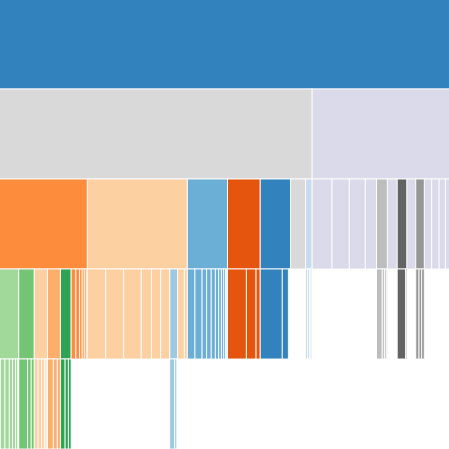
\includegraphics[width=\thumbnailWidth]{figs/visThumbnails/icicle.png}}
      & \parbox[c]{\descWidth}{\descPadding
        1 Dimension, Hierarchical (rectangles) \\
        1 Measure (rectangle length) \\
        Optionally: \\
        Picking interaction (click on rectangle)
      \descPadding} \\ \hline

    TreeMap

      & \parbox[c]{\thumbnailWidth}{\centering 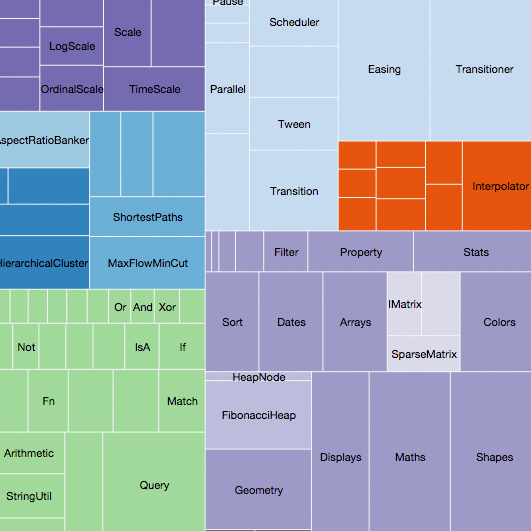
\includegraphics[width=\thumbnailWidth]{figs/visThumbnails/treemap.png}}
      & \parbox[c]{\descWidth}{\descPadding
        1 Dimension, Hierarchical (rectangles) \\
        1 Measure (rectangle area) \\
        Optionally: \\
        Picking interaction (click on rectangle)
      \descPadding} \\ \hline

    Streamgraph

      & \parbox[c]{\thumbnailWidth}{\centering 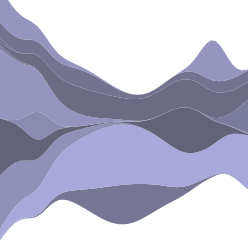
\includegraphics[width=\thumbnailWidth]{figs/visThumbnails/streamgraph.png}}
      & \parbox[c]{\descWidth}{\descPadding
        2 Dimensions, (Time, streams) \\
        1 Measure (stream thickness) \\
        Optionally: \\
        Picking interaction (click on stream), or
        Picking interaction (click on time), or
        Brushing interaction (across Time)
      \descPadding} \\ \hline

%streamgraph
%sunburst

%brushing
%donut
%embeddedGeoVisualizations
%picking
%pie
%stackedArea
%stackedBars
%table
%temporalBrushing
%treemap
  \end{tabular}
\end{table*}

\section{Data Sources}

There are numerous rich data sources on the Web that are suitable for import into the Universal Data Cube framework for visualization. So far only a few data sets have been actually imported, however many have been evaluated and identified as candidates. Some data sources provide archives of historical data, while others are vastly large and expose the data via a Web API. Crowdsourcing platforms also present immense potential for finding data sources and curating data.

The Pew Global Religious Landscape data set provides data about religious composition by country. This data set covers dimensions of Time (only the 2010 slice is provided), Space (countries), and Religion. The measure can be modeled as Population, as the addition of the Religion dimension effectively is a filter through which to view the population of a place. This data set can be enhanced by integration with a data set providing population data for each country of the World in 2010.

For each country, it is possible to visualize the data cube slice for that country as a bar chart in which each bar represents a religion. Therefore a visualization with linked views can be assembled in which picking interaction in a choropleth map can drive the country used as input for the bar chart. Clicking on each country would show its religious profile as a bar chart. This linked visualization would use the map to visualize and navigate the Space dimension, and the bar chart to visualize the Population measure by the Religion dimension. Together, the map and bar chart could visualize a data cube with 2 Dimensions (Space, Religion) and 1 Measure (Population). The original data cube included the Time dimension as well, which effectively gets eliminated by taking only the 2010 slice as input. If historical data were available for each year, a line chart could be paired with the linked visualization to visualize and navigate the Time dimension.

The Religious Landscape data set can also be visualized as bar charts (or pie charts, or donut charts) overlaid on a geographic map. The bar charts can be squares with area representing population. Each bar within the square represents a religion. By pairing size of the bar chart with population, area corresponds to quantity of people accurately. In other words, each pixel on the screen inside a bar represents a fixed number of people. Visually, this makes sense because the human visual system naturally experiences and assesses sizes of things based on their area. \cite{tufte1983visual} Pie charts could also be overlaid on a geographic map to express the same information.

Whether pie charts or bar charts, the embedded visualizations are at risk of occluding each other when plotted directly centered at the centroid of their corresponding regions. This can be overcome by using a force directed layout that repels embedded visualizations away from one another such that each is fully shown and not occluded by others. A similar technique has been used previously in cartography to produce cartograms based on circles (Dorling Cartogram) and squares (Demers Cartogram) \cite{tobler2004thirty}.

Note that the geographic visualization overlay presents the same information as the above described linked map and bar chart interactive visualization. Rather than clicking on a country, the user can now just look at the center of any given country on the map to assess its religious breakdown. In this way, the geographically overlaid visualizations communicate more information at a time than the linked views. 

The geographic bar chart visualization could also be augmented by a line chart if historical data is also available. The line chart could visualize the Time Dimension as a streamgraph chart showing global religious breakdown over time. Picking interaction for years in the streamgraph can define the Time slice used as input to the other visualizations. This is one example of the general case that adding another visualization with picking interaction can effectively add another dimension to the data space users are capable of navigating with the visualization interface.


%Data APIs e.g. World Bank, CDC, WHO
%
%MDG
%
%BLS
%
%Eurostat
%
%Census
%
%ACS
%
% http://www.worldmapper.org/data.html



DBPedia is a knowledge graph representation of Wikipedia. DBPedia data is represented using RDF (Resource Description Framework), the World Wide Web Consortium standard knowledge graph representation for the Semantic Web \cite{klyne2006resource}. In DBPedia, each Wikipedia Page about an entity is classified according to the DBPedia Ontology \cite{bizer2009dbpedia}. Resources in DBPedia can be aggregated along the DBPedia Ontology to produce a data cube that can be visualized. For example, one could visualize the count of resources for each ontology class using a Sunburst or Icicle visualization. Since resources have (lat, long) coordinates and associated dates, they can also be aggregated along Space and Time.

OpenStreetMap (OSM) is a community maintained crowdsourced geographic data repository \cite{haklay2008openstreetmap}. The OSM database contains entities of numerous types including roads, points of interest, educational institutions, churches, buildings, military bases, shops, and public transit stations \cite{osmMapFeatures}. Any of these types can be counted across geographic space and used as indicators. For example, the number of buildings can be used to approximate population at a high resolution. Map features can also be aggregated by type and visualized to show the breakdown of the database.

The 2014 global Ebola outbreak is being monitored closely. Structured data about the outbreak is available and updating every day. This data provides measures ``number of Ebola deaths'' and ``number of Ebola cases'' for each affected West African nation for each day since the outbreak began. The New York Times published a graphical piece including a small multiples visualization of Ebola \cite{nytEbola}. This is a topic prominent in the news today. A dynamically updating visualization for this data would be indispensable for journalists and decision makers alike.

The Global Terrorism Database provides historical data about terrorist activities such as attacks with their time, place, and number of deaths. With daily news on ISIL (Islamic State of Iraq and the Levant), this live updating data set is a valuable resource for many people including journalists, policy makers, or anyone interested in learning about terrorist related events. This data can be aggregated into a data cube covering dimensions Time (nested structure of years, months, days), Space (geographic region), and providing the measure of number of deaths. This data could be visualized as a linked line chart and choropleth map. Picking in the line chart slices data used as input to the choropleth map. Zooming in the choropleth map dices the data shown in the line chart. This is similar to the linked view visualization of population described in figure \ref{fig:choropleth}.


\begin{figure}
  \centering
  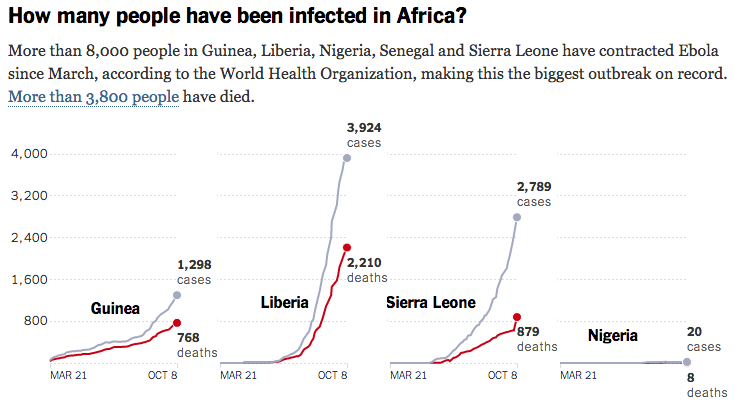
\includegraphics[width=\figureWidth]{figs/nytEbolaLines.png}
  \caption [New York Times Ebola Visualization]{ A small multiples line chart visualization of the 2014 Ebola outbreak in West Africa published by the New York Times \cite{nytEbola}. This visualization shows the number of Ebola cases and deaths by day by region.}
  \label{fig:nytEbolaLines}
\end{figure}

Crowdsourcing may also be a promising approach for collecting and curating data. Each combination of region, time and measure can be formulated as an English question, such as ``What was the GDP of India in 1970?''. Crowdsourcing platforms such as Amazon Mechanical Turk and Crowdflower can potentially be utilized to collect data. Workers may also be asked to enter the URL from which they found the data value. These URLs can be used to glean the structure of what is covered by various data sources, which can in turn be used to suggest URLs to future workers for certain regions of the data cube structure. Using this approach, it may be possible to develop an automated service that collects requested data on demand. Crowdsourcing techniques can also be used to refine the quality of the data collected.

\section{A Grammar of Graphics Approach}
A system based on named visualizations (e.g. "Scatter Plot", "Bar Chart") allows each visualization to have their own implementation, and does work. However, this approach is limited in that it does not take advantage of the deeper structure of visualizations. Leland Wilkinson's "Grammar of Graphics" describes a language for expressing many types of visualizations using a single grammar \cite{wilkinson2005grammar}. Hadley Wickham has implemented this grammar and extended it in the R package \verb1ggplot21 \cite{wickham2010layered, wickham2009ggplot2}. A JSON-based grammar of graphics called VisJSON has also been developed \cite{vizJSON}.

Incorporating a grammar of graphics implementation into the proposed visualization platform would allow configuration of powerful and complex linked visualizations using a minimally complex structure. Each visualization on a page could be described by a grammar of graphics expression, rather than invoking a module that implements a named visualization. This kind of system would be much more elegant. One additional benefit of this organization is that when new features such as interaction techniques are implemented in the grammar of graphics engine, all visualizations immediately have the new interaction available. In a named visualization system, the interaction would need to be implemented once per visualization module.

One path to a grammar of graphics based approach within the existing reactive visualization framework is to create a grammar based solution that can express incrementally more visualizations. In this sense, it is essential to first have developed a named visualization approach, then start on the grammar of graphics approach. For example, a grammar of graphics based solution can be introduced that first can generate a scatter plot, then a bar chart, then a pie chart, then a stacked bar chart. As the implementation grows in completeness, named visualizations can be incrementally replaced with expressions in the grammar.

\section{Final Thoughts}
The hoped for eventual impact of this work is to enable common everyday people to understand their world better through data visualization. By providing a basis on which complex interactive visualization systems can be built and tailored to the data at hand, this work paves the way for future researchers and developers to create visualizations that represent data clearly and can be understood by many. Whether seen on a news site, included in a corporate report, or developed for scientific research, the impact of interactive data visualizations on users is immense and immediate.

If over time more and more data sets are imported into the UDC framework, made available publicly, and visualized, the phenomenal world will be covered more and more thoroughly by the reach of digitized information and visual presentations of it. Data and visualizations about various aspects of the world will become ever more commonplace, and part of common knowledge. With the advent of social media, sharing visualizations over the Web allows them to reach huge audiences very quickly. As time passes, select visualizations may become iconic, such as Minard's map of Napoleon's march has already. Such visualizations could eventually become ``required reading'' for academic courses of study. As such they could be integrated as interactive visualizations within E-Books being consumed via tablets or laptops.

There is a concept called ``Mirror World'' envisioned by Computer Science Professor David Gelerntner in which computers attain a kind of digital mirror of reality \cite{gelernter1991mirror}. This dissertation introduces a means to define and populate a mirror world in terms of data cube aggregates, and also introduces a means to present the resulting data based view of the world via interactive visualizations. The hierarchical regions of Time and Space delineated by humans serve as the skeleton for our mirror world, and any measurable quantitative value that varies across Time, Space and additional dimensions can be incorporated into this mirror world. As more data becomes available, shedding digital light on the mysterious analog world, people will be able to understand the world around them more clearly through data visualization.
